\documentclass[conference]{IEEEtran}
\IEEEoverridecommandlockouts
% The preceding line is only needed to identify funding in the first footnote. If that is unneeded, please comment it out.
\usepackage{cite}
\usepackage{amsmath,amssymb,amsfonts}
\usepackage{algorithmic}
\usepackage{graphicx}
\usepackage{textcomp}
\usepackage{xcolor}
\def\BibTeX{{\rm B\kern-.05em{\sc i\kern-.025em b}\kern-.08em
    T\kern-.1667em\lower.7ex\hbox{E}\kern-.125emX}}
\begin{document}

\title{Evaluating Recommender Systems for Digital Library Datasets\\
% {\footnotesize \textsuperscript{*}Note: Sub-titles are not captured in Xplore and should not be used}
%\thanks{Identify applicable funding agency here. If none, delete this.}
}

\author{
\IEEEauthorblockN{1\textsuperscript{st} Ákos Lévárdy}
\IEEEauthorblockA{\textit{Faculty of Informatics and Information Technologies} \\
\textit{Slovak university of technology in Bratislava}\\
Bratislava, Slovakia \\
xlevardya@stuba.sk}
\and
\IEEEauthorblockN{2\textsuperscript{nd} Jan Lang}
\IEEEauthorblockA{\textit{Faculty of Informatics and Information Technologies} \\
\textit{Slovak university of technology in Bratislava}\\
Bratislava, Slovakia \\
jan.lang@stuba.sk}
\and
\IEEEauthorblockN{3\textsuperscript{rd} Milada Omachelova}
\IEEEauthorblockA{\textit{Faculty of Informatics and Information Technologies} \\
\textit{Slovak university of technology in Bratislava}\\
Bratislava, Slovakia \\
milada.omachelova@stuba.sk}
\and
\IEEEauthorblockN{4\textsuperscript{rd} Pavol Batalik}
\IEEEauthorblockA{\textit{Faculty of Informatics and Information Technologies} \\
\textit{Slovak university of technology in Bratislava}\\
Bratislava, Slovakia \\
pavol.batalik@stuba.sk}
}

\maketitle

\begin{abstract}
As digital content continues to grow rapidly, users face increasing difficulty in finding relevant information efficiently—especially within large-scale digital libraries. Recommender systems help address this challenge by delivering personalized suggestions that improve user experience and reduce information overload. This study focuses on evaluating content-based recommender systems tailored for digital library datasets. These systems analyze textual data from books to generate recommendations based on similarities in content features. The goal is to compare algorithms such as TF-IDF, LSA, GloVe, FastText and Sentence-BERT under different settings, assessing their effectiveness in generating Top-N recommendations. To provide a comprehensive evaluation, the study uses multiple performance metrics including similarity, diversity, confidence, and coverage, while also measuring execution time and memory usage. Our findings show that while transformer-based and neural embeddings (e.g., FastText, BERT) achieve higher similarity scores, traditional methods like LSA strike a better balance between similarity, diversity, and efficiency. These results provide actionable insights into algorithm selection for scalable recommendation systems in academic libraries.
\end{abstract}





\begin{IEEEkeywords}
Recommender System, Content-Based, Evaluation, Performance Metrics, Digital Library
\end{IEEEkeywords}



\section{Introduction}

Making decisions in today’s digital world is not always easy. Whether choosing a product, a movie, or a travel destination, people are often faced with an overwhelming number of options and varying levels of information and trustworthiness. While some users know exactly what they are looking for and seek immediate answers, others are open to exploring new possibilities and expanding their knowledge \cite{Blanco201333}.
\textbf{Recommendation Systems (RS)} are designed to ease this process by predicting useful items, comparing them, and suggesting the most similar options based on user preferences. These systems have become essential tools for reducing information overload, especially with the rapid growth of big data \cite{Haruna2017}. By analyzing large volumes of textual data, they aim to understand users’ preferences and generate personalized recommendations \cite{Yan2024}.
The task of providing users with available options that match their needs and interests is increasingly important in today’s consumer society. Without a starting point—such as a list of relevant suggestions—users may feel overwhelmed or even choose to give up entirely. For example, trying to pick a movie from scratch without any recommendations can lead to decision fatigue. Recommender systems help prevent this by offering tailored suggestions that guide the user and reduce decision friction.
%It’s also important to recognize the dual perspective from which recommendation systems operate \cite{Ricci20221}. On one hand, service providers aim to use these systems to sell more items, improve user satisfaction, or better understand customer behavior. On the other hand, from the user’s viewpoint, RS assist in discovering suitable items, recommending sequences, or even influencing others' decisions.
The core goal of RS is to personalize content and improve user experience by recommending books, movies, music, products, and more. For example, in a digital library which has loads of books available online, a recommender system might suggest books or even specific paragraphs based on a user’s reading history \cite{Zangerle2023}. These systems function by identifying relationships between users and the items they interact with—such as preferring historical documentaries over action films \cite{pub.1022525812}.
Various techniques are used to achieve this personalization. Collaborative filtering recommends items based on similar users’ preferences, while content-based filtering analyzes item features like genre or keywords. Hybrid approaches combine both for more accurate results \cite{Aymen2022896}. Regardless of the method, the aim is to help users discover relevant content they might not have found on their own.
That said, information systems must also account for the fact that user preferences can change over time. This phenomenon, known as concept drift, refers to unexpected changes in data patterns or behaviors that can significantly affect the system’s prediction accuracy \cite{Sun2024}. Recommender systems need to be adaptive in order to stay effective over long periods.
Recommendation systems differ from search engines, although both are used to navigate large amounts of information. While search engines retrieve content based on keywords, recommender systems make predictions based on user behavior and inferred interests \cite{De_Nart201484}.
This paper focuses on evaluating and comparing different recommendation algorithms for suggesting books and their parts based on textual content. Algorithms such as TF-IDF, LSA, and BERT will be tested to assess how effectively they generate recommendations. Evaluation will consider metrics like similarity, diversity, confidence, and coverage \cite{Gunawardana2022547}, along with performance factors such as execution time or memory usage.
%
%
%
The rest of the paper is organized as follows. Section 2 compares three well-known e-Learning systems and presents findings related to collaboration on tasks within the course, emphasizing the importance of clear communication of requirements through the public disclosure of tasks. Section 3 explains the educational content identification promotion based on the Event Database platform as proposed solution to achieve better performance in exams. Section 4 describes the setting of the experiment space. Section 5 concludes the paper and indicates some possibilities for further work.
%
%
%
\section{Understanding Recommendation Systems}
Recommending items can be done in a variety of ways. Several types of recommendation systems exist, and their methods of operation differ \cite{Roy2022}. Here are the different recommendation system types:\\
%
%
%\textbf{Content-Based Filtering} works in a way that it creates user profiles and suggests the individual items or products based on the users past choices with similar items. The items have various features and characteristics which connect them.\\
\textbf{Content-Based Filtering} recommends items based on a user's previous choices or interactions by finding similarities between the items the user has shown interest in and other items with similar features (e.g., genre, attributes, keywords) \cite{pub.1034486657}.
This approach focuses primarily on the item's characteristics rather than relying on other users' preferences.\\
\textbf{Collaborative Filtering} relies more on preferences of other users and their behaviour. The point is that users who had similar interests before will have them again in the future for new items. This technique relies on having user related data, feedback that could be either explicit (ratings) or implicit (passive user behaviour) \cite{NILASHI2018507}.
%
\begin{figure}[!htb]
\centering
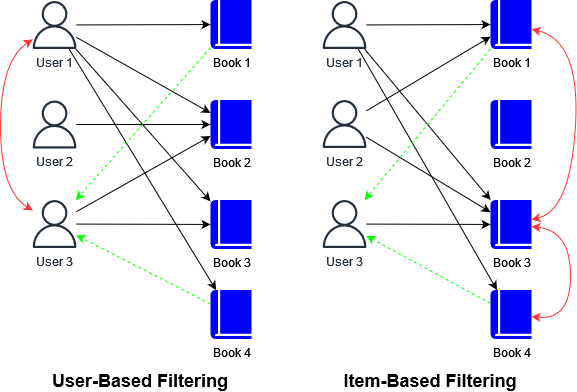
\includegraphics[width=3.5in]{img/collaborative_example.png}
\caption{Memory-based CF recommendation.}
\label{fig:collaborative_example}
\end{figure}\\
%
\textbf{Knowledge-Graphs} use a network of data where items are linked through their features. Showing how items relate to one another and connecting them with more information \cite{Imene2022488}.
%
\begin{figure}[!htb]
\centering
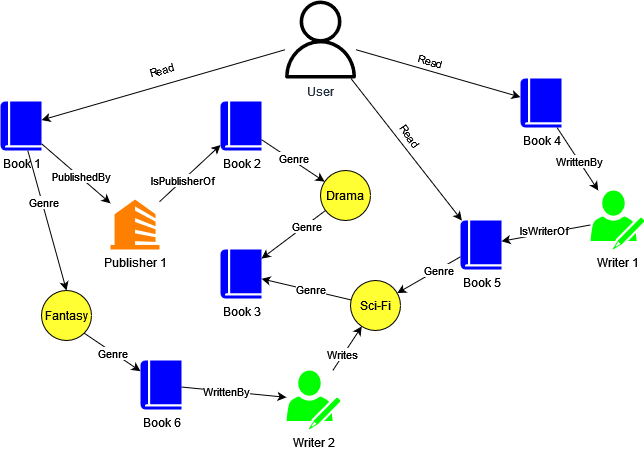
\includegraphics[width=3.5in]{img/knowledge_graph_example.png}
\caption{KG-aware recommendation.}
\label{fig:knowledge_graph_example}
\end{figure}\\
%
\textbf{Context-Aware} recommendation systems are adding contextual factors to the rating process, where the recommended item is based on the users explicit ratings, the items implicitly inferred ratings and also the contextual variables \cite{Haruna2017}. The variables for example when recommending a movie can be the location from where the user watches the movie, the time and the companion who the user watches the movie with.\\
\textbf{Demographic} recommendation systems are recommending items based on a demographic profile of the user. They categorize the users from their personal attributes and try to make user stereotypes \cite{Burke2002331}.\\
\textbf{Utility-Based} systems generate the recommendations by computing the utility of each item for the user. The utility of an item refers to how valuable it is to a user and is calculated using a utility function which combines different factors of the user's preferences \cite{Burke2002331}.\\
\textbf{Deep Learning-Based} are trying to find complex patterns in the users behaviour and the items features using deep learning algorithms and neural networks. These models can locate hidden links and can offer highly customized recommendations.\\
\textbf{Hybrid methods} try to combine the useful characteristics of both collaborative filtering and content-based filtering methods. They take into account both the users past preferences and the preferences of other people who might share the users taste \cite{melville:aaai02}. \\
%
The most popular techniques used are the Collaborative Filtering, Content-Based Filtering and the Hybrid method \cite{pub.1072601078}. This paper will focus on comparing different algortihms that are used for Content-Based Filtering, since trying to recommend books and their paragraphs in digital libraries relies on the textual content of them.




\section{System Decription}
\subsection*{Extracting Information and Building a Dataset}
First, the books were extracted from the digital library and stored as individual JSON files. Each file contained the entire data of a single book, further segmented into sentences, pages, and paragraphs for flexibility in experimentation.
For the full-text analysis, a dataset of 45k paragraphs was created. The average paragraph length was approximately 60-70 words, with the longest paragraph consisting of 2000 words.\\
In addition to the extracted book paragraphs, a publicly available dataset titled \textit{Books Details Dataset}, which was scraped from Goodreads %\cite{goodreads_kumar_2022} 
was also used in the experiments. This dataset includes metadata for over 13,000 books, such as title, author, genres, ratings, and textual descriptions averaging approximately 163 words. These summaries were treated similarly to paragraphs during preprocessing and recommendation, allowing models to be tested on both short- and long-form content for robustness and comparison.

\subsection*{Models selected for the Evaluation}
In the context of academic book recommendations, a variety of content-based algorithms can be used to extract meaningful patterns and relationships from textual data. These algorithms differ in their approach to representing and analyzing documents, words and textual data. The selected algorithms represent a diverse spectrum of CB recommendation approaches, from classical sparse models to modern transformer-based embeddings:
%
\begin{itemize}
    \item \textbf{TF-IDF and BoW} are \emph{sparse count-based models}, included as traditional baselines for textual similarity. They are fast, interpretable, and serve as a reference point for evaluating more advanced models.
    \item \textbf{LSA} is a \emph{matrix factorization technique} that captures latent semantic structures in documents. It adds a dimension-reduction perspective to the evaluation.
    \item \textbf{GloVe and FastText} are \emph{pretrained static word embedding models}, chosen for their ability to encode semantic meaning into dense vectors. FastText also includes subword information, allowing it to handle out-of-vocabulary words effectively.
    \item \textbf{Sentence-BERT (all-MiniLM-L6-v2)} is a \emph{transformer-based deep learning model} specifically optimized for sentence-level semantic similarity. It represents a state-of-the-art approach in content-based recommendation and is included to benchmark modern deep embedding techniques.
\end{itemize}
%
This selection allows a fair comparison across traditional, embedding-based, and deep learning methods in terms of similarity, diversity, and computational efficiency.\\
%
To generate recommendations, each algorithm first transformed (embedded or vectorized) all paragraphs in the dataset into numerical representations according to its own architecture:
%
\begin{itemize}
    \item \textbf{TF-IDF} and \textbf{BoW} used scikit-learn's \texttt{TfidfVectorizer} and \texttt{CountVectorizer} with English stop words removed. Tokenization was based on whitespace and punctuation, with a vocabulary size capped at 5,000 most frequent terms.

    \item \textbf{LSA} began with TF-IDF vectorization and then applied \texttt{TruncatedSVD} for dimensionality reduction with 500 components, uncovering latent semantic structures across terms.

    \item \textbf{GloVe} used pre-trained 50-dimensional word embeddings from the \texttt{glove.6B.50d.txt} file, which contains word vectors trained on 6 billion tokens from Wikipedia. Tokenization was done using simple whitespace splitting, and paragraph embeddings were obtained by averaging the vectors of all matching words in the vocabulary.

    \item \textbf{FastText} was trained on the dataset using \texttt{gensim}'s implementation with the following hyperparameters: \texttt{vector\_size=100}, \texttt{window=5}, \texttt{min\_count=2}, \texttt{workers=6}, and \texttt{epochs=20}. Paragraph vectors were computed by averaging all available subword embeddings from the tokenized input.

    \item \textbf{Sentence-BERT} used the pre-trained \texttt{all-MiniLM-L6-v2} model from the \texttt{SentenceTransformers} library. The model handled tokenization and embedding internally, producing 384-dimensional sentence embeddings via mean pooling. Embeddings were computed on GPU to accelerate cosine similarity calculations.
\end{itemize}
After generating embeddings or vectors for all documents, the input paragraph was transformed using the same method. Cosine similarity was calculated between the input and all candidate paragraphs to identify the most similar items. This metric measures the angle between two vectors, with a smaller angle (closer to 1) indicating greater similarity.
%
To ensure efficiency, especially on larger datasets, the cosine similarity computations were parallelized using \texttt{joblib}. 
The sorted similarity scores were then used to return the most similar paragraphs as recommendations.\\
%
To control the quality of recommendations, only results with cosine similarity above a dynamically computed threshold were retained. This threshold was defined as a fraction (typically 50\%) of the maximum similarity score observed in a given query. The rationale behind this relative threshold was to adapt the selection to each input case and filter out weak matches while preserving the top results. Finally, the remaining candidates were sorted by similarity score, and the top-N most similar items were returned as recommendations.
%
Notably, the similarity threshold varied across models. For TF-IDF, BoW, LSA, and BERT, the default threshold of 0.5 times the maximum similarity score was used. However, FastText and GloVe produced consistently high similarity scores across most inputs, often exceeding 0.9 even for weak semantic matches. This was likely due to their dense embeddings and averaging strategies, which compress semantic differences. Therefore, stricter thresholds were applied—0.95 for FastText and 0.99 for GloVe—to avoid returning overly generic or weakly relevant results. This threshold tuning was essential to ensure the coverage metric reflected meaningful recommendations and to improve result precision in models where cosine similarity values were inflated by design.

\begin{table}[htbp]
\caption{Performance on Book Descriptions}
\centering
\begin{tabular}{|l|r|r|r|r|r|r|}
\hline
\textbf{Metric} & \textbf{TF-IDF} & \textbf{BoW} & \textbf{FT} & \textbf{GloVe} & \textbf{LSA} & \textbf{BERT} \\
\hline
Sim.      & 0.20 & 0.25 & 0.95 & 0.98 & 0.43 & 0.36 \\
Cov. (\%) & 0.34 & 0.23 & 0.53 & 0.25 & 0.12 & 0.20 \\
Conf.     & 0.95 & 0.94 & 0.99 & 1.00 & 0.93 & 0.95 \\
Div.      & 0.0027 & 0.0050 & 0.0001 & 0.0000 & 0.0055 & 0.0033 \\
Time (s)  & 3.97 & 15.26 & 49.96 & 14.88 & 13.24 & 74.46 \\
Mem (MB)  & 293  & 378 & 2003 & 421 & 745 & 1227 \\
\hline
\end{tabular}
\label{tab:desc}
\end{table}

%\begin{table}[htbp]
%\caption{Metrics Comparison by Algorithm – Book Descriptions}
%\centering
%
%\begin{tabular}{|l|c|c|c|c|c|c|}
%\hline
%\textbf{Metric} & \textbf{TF-IDF} & \textbf{BoW} & \textbf{FastText} & \textbf{GloVe} & \textbf{LSA} & \textbf{BERT} \\
%\hline
%Avg Similarity      & 0.196   & 0.254   & 0.945   & 0.981   & 0.425   & 0.359   \\ \hline
%Coverage (\%)       & 0.34    & 0.23    & 0.53    & 0.25    & 0.12    & 0.20    \\ \hline
%Confidence          & 0.95279 & 0.93772 & 0.99023 & 0.99787 & 0.93325 & 0.94778 \\ \hline
%Diversity           & 0.00270 & 0.00499 & 0.00010 & 0.00000 & 0.00551 & 0.00334 \\ \hline
%Elapsed Time (s)    & 3.973   & 15.256  & 49.959  & 14.888  & 13.248  & 74.456  \\ \hline
%Memory Usage (MB)   & 293.49  & 378.45  & 2002.80 & 420.78  & 744.64  & 1227.44 \\ \hline
%CPU Time (s)        & 1.729   & 0.809   & 44.964  & 10.314  & 8.179   & 103.399 \\ \hline
%\end{tabular}
%\label{tab12}
%\end{table}
%
%
%

\begin{table}[htbp]
\caption{Performance on Paragraph Dataset}
\centering
\begin{tabular}{|l|r|r|r|r|r|r|}
\hline
\textbf{Metric} & \textbf{TF-IDF} & \textbf{BoW} & \textbf{FT} & \textbf{GloVe} & \textbf{LSA} & \textbf{BERT} \\
\hline
Sim.      & 0.28 & 0.19 & 0.94 & 0.99 & 0.30 & 0.35 \\
Cov. (\%) & 0.06 & 1.30 & 15.32 & 21.52 & 1.20 & 9.29 \\
Conf.     & 0.95 & 0.97 & 0.99 & 1.00 & 0.95 & 0.95 \\
Div.      & 0.0027 & 0.0007 & 0.0001 & 0.0000 & 0.0027 & 0.0025 \\
Time (s)  & 15.20 & 3.72 & 13.37 & 4.65 & 3.50 & 21.21 \\
Mem (MB)  & 293 & 203 & 1193 & 344 & 425 & 1141 \\
\hline
\end{tabular}
\label{tab:para}
\end{table}

%\begin{table}[htbp]
%\caption{Metrics Comparison by Algorithm – Paragraphs}
%\centering
%\resizebox{\textwidth}{!}{%
%\begin{tabular}{|l|c|c|c|c|c|c|}
%\hline
%\textbf{Metric} & \textbf{TF-IDF} & \textbf{BoW} & \textbf{FastText} & \textbf{GloVe} & \textbf{LSA} & \textbf{BERT} \\
%\hline
%Avg Similarity      & 0.276   & 0.193   & 0.939   & 0.989   & 0.297   & 0.349   \\ \hline
%Coverage (\%)       & 0.06    & 1.30    & 15.32   & 21.52   & 1.20    & 9.29    \\ \hline
%Confidence          & 0.95279 & 0.97252 & 0.99032 & 0.99799 & 0.95164 & 0.95391 \\ \hline
%Diversity           & 0.00270 & 0.00074 & 0.00010 & 0.00000 & 0.00273 & 0.00246 \\ \hline
%Elapsed Time (s)    & 15.206  & 3.722   & 13.373  & 4.646   & 3.501   & 21.217  \\ \hline
%Memory Usage (MB)   & 293.49  & 202.89  & 1193.43 & 344.33  & 424.85  & 1141.38 \\ \hline
%CPU Time (s)        & 7.230   & 0.275   & 11.821  & 3.210   & 2.041   & 27.757  \\ \hline
%\end{tabular}
%}
%\end{table}


\section{Experimental Results for Evaluation}

Each algorithm was evaluated using 10 independent test runs, where each run used a different input item. For paragraph-level evaluation, 10 distinct paragraphs from the extracted book texts were used as inputs. For the description-level evaluation, 10 different book summaries from the Goodreads dataset~%\cite{goodreads_kumar_2022} 
were selected. The same set of 10 inputs was used across all algorithms to ensure consistency and fairness.

In each run, the algorithm generated recommendations from the corresponding dataset (paragraphs or descriptions), and the similarity scores of these recommendations were used to compute performance metrics. The final metric values for each algorithm were obtained by averaging the scores across all 10 runs.

The following metrics were calculated:
\begin{itemize}
    \item \textbf{Average Similarity}: Mean cosine similarity between the input item and its Top-N recommendations.
    \item \textbf{Item Coverage}: Percentage of unique recommended items across all runs, indicating how broadly the model explores the dataset.
    \item \textbf{Confidence}: Inverse of the standard deviation of similarity scores. A lower variance indicates more confident (i.e., stable) recommendations.
    \item \textbf{Diversity}: Variance of similarity scores among the recommended items. Higher variance implies greater diversity within the Top-N list.
\end{itemize}

These metrics were chosen to reflect both the quality and consistency of the recommendations, especially since explicit user feedback data was not available. Therefore, traditional recommendation metrics like Precision or Recall could not be applied. Instead, content-based internal evaluation using cosine similarity allowed for a fair, interpretable comparison of the models.












\section{Conclusions and Future Work}

This study presented a comparative evaluation of several content-based recommendation algorithms—namely TF-IDF, BoW, LSA, GloVe, FastText, and Sentence-BERT—applied to digital library data at both paragraph and book-description levels. The results demonstrate that while neural models like FastText and GloVe achieve high similarity scores, they also require significantly more computational resources. On the other hand, traditional models such as TF-IDF and BoW offer fast and lightweight alternatives, but with reduced accuracy.

LSA was shown to strike a middle ground between relevance, diversity, and efficiency, making it a viable option for systems where balance across these factors is important. Sentence-BERT provided strong performance with moderate similarity and higher processing overhead, suggesting its potential for systems where context-rich recommendations are critical.

Overall, the analysis highlights clear trade-offs between recommendation quality, computational cost, and item coverage. These insights offer practical guidance for selecting and deploying content-based recommendation algorithms in academic or large-scale library systems. By aligning system requirements—such as speed, accuracy, or breadth of exploration—with algorithmic strengths, developers can build more effective and scalable recommender systems tailored to digital content.\\

Future research could expand the evaluation by including additional state-of-the-art models beyond the ones tested in this study. Transformer-based architectures such as RoBERTa, DistilBERT, or retrieval-augmented models like RAG and ColBERT may offer improved performance, especially on complex or ambiguous queries. These models are designed to capture deeper contextual relationships and may enhance both relevance and semantic precision in recommendations.

Another promising direction is to experiment with hybrid approaches that combine content-based filtering with collaborative signals (e.g., user ratings or interaction history), enabling systems to adapt dynamically to individual user preferences. This could lead to more personalized and context-aware recommendations.

From a technical perspective, optimizing runtime and memory efficiency, particularly for large-scale datasets, could be achieved through model distillation, approximate nearest neighbor techniques, or embedding quantization. Additionally, evaluating models across more diverse content types and multilingual datasets would help assess their generalizability and robustness.



\ifCLASSOPTIONcaptionsoff
  \newpage
\fi

\bibliographystyle{plain} 
\bibliography{literature}

\graphicspath{ {./fig/} }

\end{document}
